\subsection{Exercises 2-4}

\num Provide an example (in pseudocode, with explanations) of a batch processing pattern where OpenMP and CUDA are used together to distribute work among multiple GPUs.

\begin{tcolorbox}
	\begin{minted}[autogobble]{cpp}
        int deviceCount;
        cudaGetDeviceCount(&deviceCount);
        std::vector<cudaStream_t> streams(deviceCount);
        
        #pragma omp parallel for num_threads(deviceCount)
        for(int dev = 0; dev < deviceCount; ++dev) { 
            // for each GPU in the system:
            cudaSetDevice(dev);
            cudaStreamCreate(&streams[i]); // use a stream for data transfers
            // Allocate, initialize and transfer memory
        }

        #pragma omp parallel for num_threads(deviceCount)
        for(int dev = 0; dev < deviceCount; ++dev) {
            cudaSetDevice(dev);
            kernel<<<gridDim, blockDim, streams[i]>>>(...);
        }
    \end{minted}
\end{tcolorbox}

\num Provide an example (in pseudocode, with explanations) of an application that uses OpenMP instead of CUDA to offload computation on a GPU.

\begin{tcolorbox}
	\begin{minted}[autogobble]{cpp}
        // Offload the following region to a GPU, 
        // transfer contents of a,b,c,d
        #pragma omp target map(a, b, c, d) {
            // use multiple GPU threads to parallelize this loop
            #pragma parallel for 
            for (i = 0; i < N; i++) {
                a[i] = b[i] * c + d;
            }
        }
    \end{minted}
\end{tcolorbox}

\num Describe the trade-offs that can be explored in the design space created by the Halide scheduling directives.

\begin{tcolorbox}
	The Halide scheduling directives navigates the trade-off between \textbf{locality}, \textbf{parallelism}, and \textbf{redundant computation} without altering the algorithm's correctness.

	Halide solves these trade-offs by decoupling the algorithm (what to compute) from the schedule (how to execute it). Allows you to write the mathematical definition once and then use scheduling directives to manipulate the execution strategy instantly:

	\begin{itemize}
		\item Re-compute values on the fly to save memory bandwidth; or
		\item compute them once and store them, which avoids redundant math but increases memory traffic; or
		\item The "sweet spot" where you compute small tiles of data just before they are needed by the consumer loop, fitting them into the cache.
	\end{itemize}
\end{tcolorbox}

\num Provide at least two examples of situations where a combination of different parallel programming languages is used.

\begin{tcolorbox}
	A common approach is MPI + OpenMP, used in supercomputing clusters where MPI manages communication between distinct computing nodes while OpenMP parallelizes the workload within each node.

	Another example is OpenMP + CUDA, used in heterogeneous systems where the CPU uses OpenMP to manage threads and data distribution, while offloading parallel compute-intensive kernels to the GPU via CUDA.
\end{tcolorbox}

\num Consider the following DFG and HLS schedule obtained with the list-based algorithm. What can you infer about the constraints on resources?

\begin{figure}[H]
	\centering
	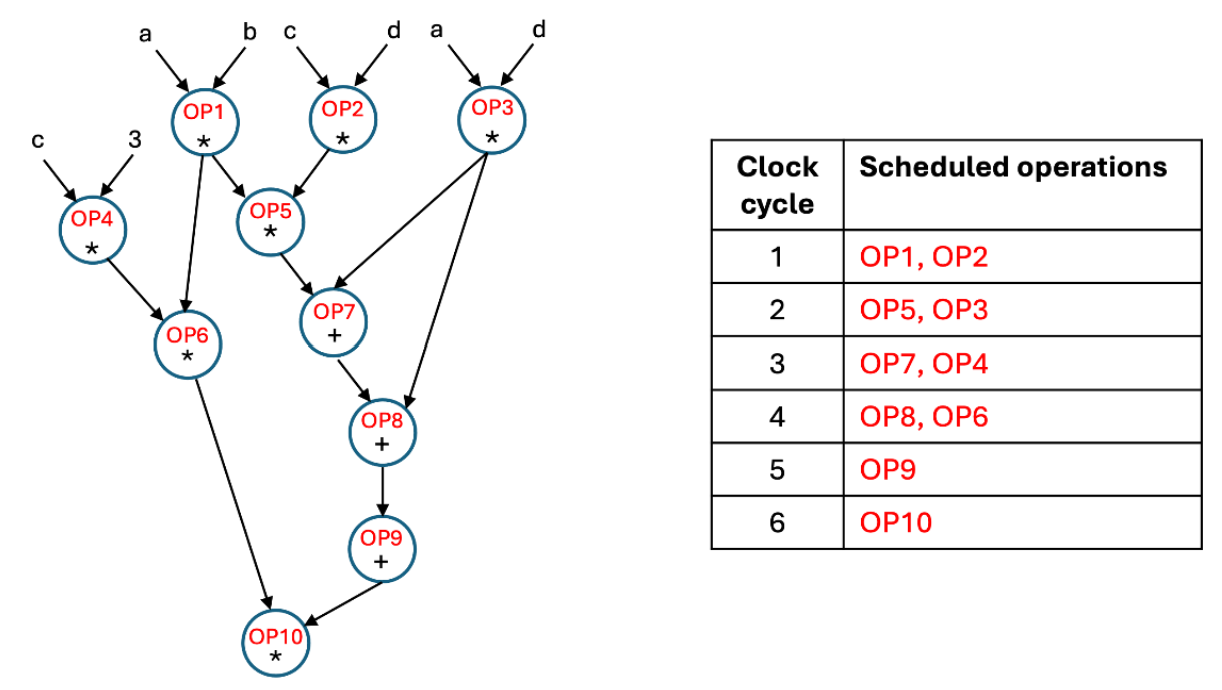
\includegraphics[width=0.7\textwidth]{images/dfg-hls.png}
\end{figure}

\begin{tcolorbox}
	The system is constrained by 2 multiplier, and at least 1 adder.
	We can tell because OP1, OP2, OP3, OP4 are all independent, yet they are not executed together (at most 2 multiplier operations
\end{tcolorbox}

\num How does the schedule from the previous question change if the available resources are 4 multipliers and 2 adders (all with 1 clock cycle latency)?

\begin{tcolorbox}
	\begin{center}
		\begin{tabular}{|c|l|l|}
			\hline
			\textbf{Clock Cycle} & \textbf{Scheduled Operations} \\ \hline
			1                    & OP1, OP2, OP3, OP4            \\ \hline
			2                    & OP5, OP6                      \\ \hline
			3                    & OP7                           \\ \hline
			4                    & OP8                           \\ \hline
			5                    & OP9                           \\ \hline
			6                    & OP10                          \\ \hline
		\end{tabular}
	\end{center}
\end{tcolorbox}

\num When is \texttt{cudaSetDevice()} used?

\begin{tcolorbox}
	\texttt{cudaSetDevice()} is used in multi-GPU environments to explicitly select which graphics card the current CPU thread should issue commands to.

	By default, a host thread operates on Device 0; if a system has multiple GPUs (e.g., Device 0 and Device 1), a developer must call cudaSetDevice(1) to switch the current thread's context to the second GPU before allocating memory or launching kernels on it.

	This setting is thread-local, meaning different CPU threads can simultaneously control different GPUs by calling this function with different device IDs.
\end{tcolorbox}

\num Describe the effect of the following OpenMP pragma:

\begin{minted}[autogobble]{text}
    #pragma omp target map(a,b)
\end{minted}

\begin{tcolorbox}
	This pragma instructs the compiler to offload the execution of the following code block to a target device (such as a GPU). The \texttt{map(a, b)} clause manages the data movement between the host (CPU) and the device: it allocates memory for variables \texttt{a} and \texttt{b} on the device, copies their values from Host to Device before the code executes, and copies the modified values back from Device to Host after the execution finishes.
\end{tcolorbox}

\num A Domain-Specific Language provides productivity and performance at the expense of generality. Is this statement true or false? Explain.

\begin{tcolorbox}
	\textbf{TRUE}.

	A Domain-Specific Language (DSL) explicitly sacrifices generalitynto optimize for a narrow purpose. By restricting the language's semantics, the compiler gains a deeper understanding of the code's intent, enabling it to perform aggressive domain-specific optimizations that maximize performance.

	Simultaneously, productivity improves because the language exposes high-level primitives that closely match the domain's model, allowing developers to describe what they want to compute rather than how to implement the low-level details.
\end{tcolorbox}

\num Describe the ASAP scheduling algorithm.

\begin{tcolorbox}
	The ASAP (As Soon As Possible) scheduling algorithm assigns every operation to the earliest possible clock cycle allowed by its data dependencies (assuming unlimited hardware resources).

	An operation is scheduled immediately after its latest predecessor has finished. While this guarantees the theoretical minimum possible total execution time (latency), it tends to creates a spike in resource usage at the beginning of the execution (often requiring more functional units than a real physical chip possesses).
\end{tcolorbox}

\num If we want to copy 3000 bytes of data from host array \texttt{h\_A} (\texttt{h\_A} is a pointer to element 0 of the source array) to device array \texttt{d\_A} (\texttt{d\_A} is a pointer to element 0 of the destination array), what would be an appropriate API call for this in CUDA?

\begin{tcolorbox}
	\begin{minted}[autogobble]{text}
        cudaMemcpy(d_A, h_A, 3000, cudaMemcpyHostToDevice);
    \end{minted}
\end{tcolorbox}

\num How is error handling implemented in a CUDA host program to check whether a kernel launch has been successful?

\begin{tcolorbox}
	Because kernels launch asynchronously and return \texttt{void}, the host program cannot directly check a return value for success. Instead, it must:

	\begin{enumerate}
		\item Call \texttt{cudagetLastError()} immediately after the kernel launch to catch synchronous error; followed by
		\item \texttt{cudaDeviceSynchronize()} to force the host to wait for the GPU to finish. This ensures that runtime errors are propagated back to the host, where they can be captured and translated into readable text using
		\item \texttt{cudaGetErrorString()}.
	\end{enumerate}
\end{tcolorbox}

\num What is asynchronous memory prefetching, and when is it useful?

\begin{tcolorbox}
	\textbf{Asynchronous memory prefetching} is a latency-hiding technique where data is fetched from slow global memory into the faster cache before the execution unit actually needs it, allowing the transfer to happen in parallel with current computations.

	It is useful in \textbf{bandwidth-bound} applications, such as matrix multiplication, where the processor would otherwise spend significant cycles stalled waiting for data to arrive.
\end{tcolorbox}

\num Why is synchronization necessary when programming with the shared memory model?

\begin{tcolorbox}
	Synchronization is necessary in the shared memory model to prevent \textbf{race conditions}, which occur when multiple threads attempt to access the same memory location simultaneously without a defined order.

	Without synchronization (like locks or barriers), the final result would depend from the unpredictable timing of thread execution.
\end{tcolorbox}

\num Sometimes a parallel program can be slower than a sequential one. Is this statement true or false? Why?

\begin{tcolorbox}
	\textbf{TRUE}.

	Parallelism always introduces \textbf{overhead}, such as the time required to create threads, synchronize them (locks/barriers), and communicate data between memory spaces. If the problem size is too small, the time spent managing these parallel tasks will be more than the time effectively saved by dividing the work.
\end{tcolorbox}

\num What is a DSL?

\begin{tcolorbox}
	A \textbf{DSL (Domain SPecific Language)} is a programming language specialized to a particular application domain. It has a restricted syntax making it more efficient at their specific purpose. There are two types of DSLs:
	\begin{itemize}
		\item \textbf{External}: a completely separate language (e.g., SQL, HTML, ...).
		\item \textbf{Embedded}: built on top of another language (like C++). It uses the host syntax but exploits its flexibility (e.g., pytorch on python). This is is easier to build (e.g., uses existing compilers) but it is constrained by the syntax rules of the host language.
	\end{itemize}
\end{tcolorbox}

\num For the \textbf{work-inefficient} scan kernel based on reduction trees, assume that we have 2048 elements in the input vector, explain how to estimate the number of add operations performed.

\begin{tcolorbox}
	In the \textbf{work-inefficient} scan, the algorithm makes $\log_2(N)$ iterative steps, (depth of the tree is $\log_2 N$). In each step, the algorithm performs a parallel addition ($\approx N$ steps). Therefore, the estimation for the total work is $O(N \log N)$ which for $N = 2048$, we have about $2048 \times \log_2 2048 = 2048 \log_2 11$ add operations.

	This is considered \textit{work-inefficient} because it performs significantly more operations than the theoretical minimum of $N - 1$ achieved by a sequential scan.
\end{tcolorbox}

\num For the \textbf{work-efficient} scan kernel based on reduction trees and inverse reduction trees, assume that we have 2048 elements in the input vector, explain how to estimate the number of add operations performed in both the forward and the reverse phase.

\begin{tcolorbox}
	In the \textbf{work-efficient} scan, the algorithm consists of two phases:

	\begin{enumerate}
		\item A reduction phase: the number of active elements halves at each step ($N/2 + N/4 + \dots + 1$), forming a geometric series that sums to $N - 1$ additions.
		\item An inverse reduction phase: traverses the tree in reverse to distribute sums, also performing $N - 1$ operations.
	\end{enumerate}

	Therefore, the estimation for the total work is $O(N)$, specifically $(N - 1) + (N - 1)$. For $N = 2048$, we perform $2047 + 2047 = 4094$ add operations.
\end{tcolorbox}

\num Describe the method to qualitatively evaluate a parallel algorithm through its data flow graph.

\begin{tcolorbox}
	To qualitatively evaluate a parallel algorithm using a Data Flow Graph, you analyze the structural geometry of the graph to determine two fundamental properties:
	\begin{itemize}
		\item Work ($T_1$): the total number of nodes in the graph, which represent the total volume of computation that must be performed;
		\item Critical path ($T_\infty$): the longest chain of dependent nodes from the start to the end of the graph.
	\end{itemize}

	The qualitative evaluation comes from comparing these two properties. A graph that is \textbf{wide and shallow} indicates high Average Parallelism ($T_1 / T_\infty$), meaning the algorithm scales well because many operations are independent.

	Conversely, a graph that is \textbf{narrow and deep} indicates a sequential bottleneck where the algorithm cannot run faster even with infinite processors.
\end{tcolorbox}

\num In Halide, it is better to start scheduling the input stage of the pipeline and proceed towards the output. Is this statement true or false? Explain.

\begin{tcolorbox}
	\textbf{FALSE}.

	In Halide, the scheduling strategy is typically consumer-driven, meaning you start with the output and work backwards to the inputs. You first define the loop structure for the final output stage, and then you schedule the producer stages (the intermediate steps or inputs) relative to that output.

	This approach ensures that values are computed and stored exactly when and where the consumer needs them, maximizing data locality and register reuse, which is difficult to achieve if you schedule inputs in isolation without knowing the consumer's access pattern.
\end{tcolorbox}

\num What are the characteristics of a program that make it amenable to parallelization with multiple threads?

\begin{tcolorbox}
	A program is amenable to parallelization if it exhibits a high degree of data independence, meaning its computational tasks or loop iterations can execute simultaneously without waiting for results from one another (no loop-carried dependencies). Also, the amount of computation per task should significantly outweighs the overhead of creating threads and synchronizing them.
\end{tcolorbox}

\num What are the characteristics of a program that make it amenable to parallelization on a GPU?

\begin{tcolorbox}
	A program is amenable to GPU parallelization if it exhibits \textbf{massive data parallelism}, meaning the same instruction sequence can be applied to multiple data elements simultaneously (SIMT). Unlike CPU threads, GPU threads require regularity: computations should have consistent control flow (minimal branch divergence) and memory access patterns should be coalesced (adjacent threads reading adjacent memory addresses).

	Additionally, the program should performing many calculations for every byte of data loaded from global memory, to effectively hide the latency of fetching data and keep the many cores utilized.
\end{tcolorbox}

\num Why would a programmer intentionally apply transformations that introduce redundant computation?

\begin{tcolorbox}
	To avoid the much higher cost of communication and memory access. In parallel systems, fetching a value from another processor or global memory (latency) is often much slower than simply re-calculating that value locally.
\end{tcolorbox}

\num Compare MPI, Pthreads, OpenMP, and CUDA according to how they describe parallelism and communication (i.e., implicitly/explicitly).

\begin{tcolorbox}
	\begin{itemize}
		\item \textbf{MPI}: handles parallelism and communication \textbf{explicitly}. You have to manage exactly how many processes run and you must explicitly send and receive data between processes.
		\item \textbf{Pthreads}: you explicitly manage every single thread using the API calls, but the communication is implicit (via shared memory).
		\item \textbf{OpenMP}: The parallelism is mostly implicit, you provide high-level directives (pragmas) and the compiler implicitly manages the threads. The communication is also implicis (via shared memory).
		\item \textbf{CUDA}: the parallelism is explicit, as you have to define the grid and block dimension (\texttt{<<<grid, block>>>}). The communication can be both explicit (there are API calls to transfer data between the host and the device) and implicit (threads communicate with each others in the same kernel via global memory).
	\end{itemize}
\end{tcolorbox}
